%% start of file `template.tex'.
%% Copyright 2006-2013 Xavier Danaux (xdanaux@gmail.com).
%
% This work may be distributed and/or modified under the
% conditions of the LaTeX Project Public License version 1.3c,
% available at http://www.latex-project.org/lppl/.


\documentclass[10pt,a4paper,sans]{moderncv}        % possible options include font size ('10pt', '11pt' and '12pt'), paper size ('a4paper', 'letterpaper', 'a5paper', 'legalpaper', 'executivepaper' and 'landscape') and font family ('sans' and 'roman')

% moderncv themes
\moderncvstyle{casual}                             % style options are 'casual' (default), 'classic', 'oldstyle' and 'banking'
\moderncvcolor{blue}                               % color options 'blue' (default), 'orange', 'green', 'red', 'purple', 'grey' and 'black'
%\renewcommand{\familydefault}{\sfdefault}         % to set the default font; use '\sfdefault' for the default sans serif font, '\rmdefault' for the default roman one, or any tex font name
%\nopagenumbers{}                                  % uncomment to suppress automatic page numbering for CVs longer than one page

% character encoding
\usepackage[utf8]{inputenc}                       % if you are not using xelatex ou lualatex, replace by the encoding you are using
%\usepackage{CJKutf8}                              % if you need to use CJK to typeset your resume in Chinese, Japanese or Korean
\usepackage{float, graphicx}

% adjust the page margins
\usepackage[scale=0.85]{geometry}
%\setlength{\hintscolumnwidth}{3cm}                % if you want to change the width of the column with the dates
%\setlength{\makecvtitlenamewidth}{10cm}           % for the 'classic' style, if you want to force the width allocated to your name and avoid line breaks. be careful though, the length is normally calculated to avoid any overlap with your personal info; use this at your own typographical risks...

% personal data
\name{Ivan}{Ogasawara}
\title{Open Source Developer}                               % optional, remove / comment the line if not wanted
% \address{street and number}{postcode city}{country}% optional, remove / comment the line if not wanted; the
% \phone[mobile]{+591 69757089}                   % optional, remove / comment the line if not wanted
%\phone[fixed]{+2~(345)~678~901}                    % optional, remove / comment the line if not wanted
%\phone[fax]{+3~(456)~789~012}                      % optional, remove / comment the line if not wanted
\email{ivan.ogasawara@gmail.com}                               % optional, remove / comment the line if not wanted
\homepage{https://www.linkedin.com/in/ivan-ogasawara/}                         % optional, remove / comment the line if not wanted
%\extrainfo{http://lattes.cnpq.br/7764277601641080}                 % optional, remove / comment the line if not wanted
%\photo[64pt][0.4pt]{picture}                       % optional, remove / comment the line if not wanted; '64pt' is the height the picture must be resized to, 0.4pt is the thickness of the frame around it (put it to 0pt for no frame) and 'picture' is the name of the picture file
% \quote{Some quote}                                 % optional, remove / comment the line if not wanted

% to show numerical labels in the bibliography (default is to show no labels); only useful if you make citations in your resume
%\makeatletter
%\renewcommand*{\bibliographyitemlabel}{\@biblabel{\arabic{enumiv}}}
%\makeatother
%\renewcommand*{\bibliographyitemlabel}{[\arabic{enumiv}]}% CONSIDER REPLACING THE ABOVE BY THIS

% bibliography with mutiple entries
%\usepackage{multibib}
%\newcites{book,misc}{{Books},{Others}}
%----------------------------------------------------------------------------------
%            content
%----------------------------------------------------------------------------------
\begin{document}
%\begin{CJK*}{UTF8}{gbsn}                          % to typeset your resume in Chinese using CJK
%-----       resume       ---------------------------------------------------------
\makecvtitle

% 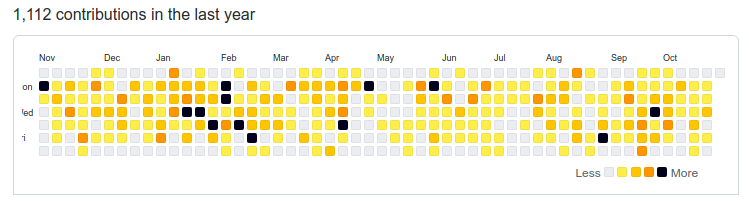
\includegraphics[width=\linewidth]{./images/github.png}

\section{Summary}
\cventry{}{In the past 19 years, I have worked as a software developer using some programming languages such as Python, C++, Javascript, PHP, VB, JAVA, ShellScript for back-end, front-end, devops and packaging. I have contributed to scientific projects as Research Software Engineering for Engineering Transportation and  Health areas. Also, I have contributed to some open source projects such as pytorch, ibis-framework, jupyter ecosystem, etc. In the past few years, I have used technologies/libraries/tools such as ibis-framework, pandas, PostgreSQL, OmniSciDB, MySQL, MSSQL, django, django-restframework, fastapi, flask, Vue.js, JQuery, conda/conda-constructor, Docker, Argo Workflow, etc. I am an Open Science enthusiast (Open Source, Open Data, and Open Access), and in the past few years, I have contributed to PyOpenSci as package reviewer and review editor. Also, I am contributing to a new community for Open Science (Open Science Labs) focused on the Latin American region}{}{}{}{}{}


\section{Education}

\cventry{2015--2016}{Transportation Engineering}{Universidade Federal de Santa Catarina}{Florianópolis/Brazil}{\textit{Master's degree (interrupted)}}{}  % arguments 3 to 6 can be left empty

\cventry{2004--2005}{Information Technology}{Faculdade Eniac}{Guarulhos/Brazil}{\textit{Specialization}}{}

\cventry{2003--2004}{Database Technology}{Faculdade Eniac}{Guarulhos/Brazil}{\textit{Associate's degree}}{}


\section{Experience}

\cventry{2018--Present}{Software Developer}{Quansight/OSBIG}{Part-time}{}{Contributed to Open Source projects such as pytorch, ibis-framework (core, omniscidb, mssql), jupyter ecosystem, omniscidb, sqlalchemy-omnisci. Worked on internal and client projects with technologies such as django, django-restframework, asyncio, bluetooth BR/EDR communication, docker, graphql, argo workflow, etc. As extra activities, I am a member of the DEI committee, where we organize internal events to promote and discuss topics related to diversity, equity, and inclusion and, I have organized and facilitated weekly meetings about compilers.}

\cventry{2017--2017}{Software Packager}{Anaconda, Inc}{Contract}{}{Acted as a software packager with conda for R libraries.}

\cventry{2016--2017}{Research Software Engineer}{Fundação para o Desenvimento Científico e Tecnológico em Saúde - Fiotec}{Contract}{}{Contributed to the development of portals for visualization of influenza and dengue incidence and estimation in Brazil. Development using technologies such as Python, Javascript, pandas, bokeh, django, flask, fiona, rasterio, PostgreSQL, MapServer, Docker, etc.}

\cventry{2016--2016}{Research Software Engineer}{Fapeu - Fundação de Amparo a Pesquisa e Extensão Universitária}{Contract}{}{Contributed to a WEB system for visco-elastic characteristics analysis of pavements in laboratory test.}

\cventry{2013--2016}{Research Software Engineer}{Fapeu - Fundação de Amparo a Pesquisa e Extensão Universitária}{Florianópolis/Brazil}{Full-time}{Analysis of international literature in order to investigate methods for supporting transport systems, such as weighing in motion (WIM) at high speed and fatigue and complex modulus essays. Development using Digital Signal Processing, Machine Learning, and High Performance Computing techniques.}

\cventry{2011--2013}{Software Developer}{Cetil Sistemas de Informática S/A}{Florianópolis/Brazil}{Full-time}{Analysis and development of management systems for public administration. Use of technologies such as .NET, VB, SQL Server, Kettle. Also, acted as Function Points accountant and reviewer.}

\cventry{2011--2011}{Software Developer}{Victory Consulting}{São Paulo/Brazil}{Full-time}{
Development of tools for the management of health insurance and life quality programs. Use of technologies such as PHP, JavaScript, jQuery, PHP Unit, Yii Framework, etc.}

\cventry{2007--2009}{Software Developer}{Prefeitura Municipal de Guarulhos}{Guarulhos/Brazil}{Full-time}{
Analysis and development of support systems for citizens and public administration. Management of GNU / Linux and Windows servers for the development team environment. Use of technologies such as MySQL, PostgreSQL, SQL Server, Apache, Tomcat, PHP, Java, VB, SVN.}

\cventry{2006--2007}{Software Developer}{Uacari Consultoria de Informática}{Guarulhos/Brazil}{Contract}{Software development using technologies such as PHP, JavaScript, and Java.}

\cventry{2005--2005}{Software Developer}{Vemac Comércio e Serviços LTDA - ME}{São Paulo/Brazil}{Full-time}{Analysis and development of systems for basic health units. Use of technologies such as VB and Microsoft SQL Server.}

\cventry{2002--2004}{Software Developer}{Colégio Eniac}{Guarulhos/Brazil}{Internship}{Systems and WEB sites development for school management. Use of technologies such as PHP, Java, Javascript, Flash, MySQL, Linux server, etc.}

\cventry{2002--2002}{Software Developer}{Quality Way}{São Paulo/Brazil}{Internship}{Development of internal system. Use of technologies such as VB6 and MS Access.}

\section{Volunteer Experience}

\cventry{2020--Present}{Software Reviewer, Review Editor}{PyOpenSci}{}{}{Acted as a software package reviewer, review editor, and recently I am a member of the editorial board.}

\cventry{2018--Present}{Founder, Director and Mentor}{Open Science Labs}{}{}{At Open Science Labs, my main tasks are to define guidance to the project in all the areas, such as: digital marketing, devops, mentoring program, training program, community management, etc. Also, I have acted in different areas such as devops, community manager, content creator, and mentor.}

\cventry{2015--2016}{Chair}{SciPy Latin America}{}{}{SciPyLA Conference 2016, held between May 16 and 20, 2016, aimed to promote: science, the adoption of information technology as a tool for scientific study and, the use of Python as the main computing tool in science (https://www.scipy.lat/conf/2016/).}

\section{Languages}
\cvitemwithcomment{Portugués}{Native}{}
\cvitemwithcomment{Español}{Fluent}{}
\cvitemwithcomment{Inglés}{Advanced}{}
\cvitemwithcomment{Italiano}{Basic}{}

%\section{Computer skills}
%\cvdoubleitem{category 1}{XXX, YYY, ZZZ}{category 4}{XXX, YYY, ZZZ}
%\cvdoubleitem{category 2}{XXX, YYY, ZZZ}{category 5}{XXX, YYY, ZZZ}
%\cvdoubleitem{category 3}{XXX, YYY, ZZZ}{category 6}{XXX, YYY, ZZZ}

%\section{Interests}
%\cvitem{hobby 1}{Description}
%\cvitem{hobby 2}{Description}
%\cvitem{hobby 3}{Description}

\section{Certificados}

\cvlistitem{Compilers. edX/Stanford (2021) }
\cvlistitem{Leading With Effective Communication, Inclusive Leadership Training. edX/Catalyst (2021)}
\cvlistitem{Parallel Computing with Dask. DataCamp (2018)}
\cvlistitem{Deep Learning in Python. DataCamp (2018)}
\cvlistitem{Machine Learning with Python. DataCamp (2018)}
\cvlistitem{Machine Learning with the Experts: School Budgets. DataCamp (2018)}
\cvlistitem{Unsupervised Learning in Python. DataCamp (2018)}
\cvlistitem{Importing \& Managing Financial Data in Python. DataCamp (2018)}
\cvlistitem{Supervised Learning with scikit-learn. DataCamp (2018)}
\cvlistitem{Introduction to Applied Biostatistics: Statistics for Medical Research. Osaka University / EDX (2017)}
\cvlistitem{Intro to Hadoop and MapReduce. Udacity (2016)}
\cvlistitem{Intro to Data Science. Udacity (2014)}
\cvlistitem{Machine Learning: Supervised Learning. Udacity (2014)}
\cvlistitem{Intro to Descriptive Statistics. Udacity (2014)}
\cvlistitem{Design of Computer Programs. Udacity (2012)}

%\section{Extra 2}
%\cvlistdoubleitem{Item 1}{Item 4}
%\cvlistdoubleitem{Item 2}{Item 5\cite{book1}}
%\cvlistdoubleitem{Item 3}{Item 6. Like item 3 in the single column list before, this item is particularly long to wrap over several lines.}

%\section{References}
%\begin{cvcolumns}
%  \cvcolumn{Category 1}{\begin{itemize}\item Person 1\item Person 2\item Person 3\end{itemize}}
%  \cvcolumn{Category 2}{Amongst others:\begin{itemize}\item Person 1, and\item Person 2\end{itemize}(more upon request)}
%  \cvcolumn[0.5]{All the rest \& some more}{\textit{That} person, and \textbf{those} also (all available upon request).}
%\end{cvcolumns}

% Publications from a BibTeX file without multibib
%  for numerical labels: \renewcommand{\bibliographyitemlabel}{\@biblabel{\arabic{enumiv}}}% CONSIDER MERGING WITH PREAMBLE PART
%  to redefine the heading string ("Publications"): \renewcommand{\refname}{Articles}

%\nocite{*}
%\bibliographystyle{plain}
%\bibliography{publications}                        % 'publications' is the name of a BibTeX file

%\begin{itemize}
%\item  Poster: OpenWIM - Open Science and Weigh in Motion Research. International Conference on Weigh-In-Motion 7. DOI: 10.13140/RG.2.2.19198.48961 (\url{https://www.researchgate.net/publication/311735715_OpenWIM_-_Open_Science_and_Weigh_in_Motion_Research})
%\end{itemize}


% Publications from a BibTeX file using the multibib package
%\section{Publications}
%\nocitebook{book1,book2}
%\bibliographystylebook{plain}
%\bibliographybook{publications}                   % 'publications' is the name of a BibTeX file
%\nocitemisc{misc1,misc2,misc3}
%\bibliographystylemisc{plain}
%\bibliographymisc{publications}                   % 'publications' is the name of a BibTeX file

\end{document}


%% end of file `template.tex'.
